\subsubsection{,,DiseaseCore" pakotne}
\subsubsection*{Multithreading}
Darba autors jau projekta plānošanas stadijā zināja, ka vēlēsies padziļināti
izpētīt un apgūt \emph{multithreaded} aplikāciajs principus, tāpēc jau pašā sākumā
centās saprast, kur projektā varētu iesaistīt dažādu asinhrono un paralēlo darbību.

Šāda nepieciešamība noveda pie sekojošās koda arhitektūrās, kuras vispārīgo
vizuālo reprezentāciju var apskatīt \ref{img:multithreaded-layout} attēlā: visa plakne, kur tiks
veikta simulācija, tiek sadalīta vienādos apakšreģionos pa \(x\) asi (\emph{Region.cs}).
Katrā apakšreģionā atrodas kaut kāda noteiktu entītiju (gan veselo, gan slimo) apakškopa.
Katrs reģions tiek piešķirts noteiktai \emph{Task}\cite{csharp:task} instancei.
Tajā brīdī, kad noteiktais entītijs šķērso \(x\) ass robežu, tad tas tiek tiek
ievietots ,,Out of bounds" buferī, kuru regulāri apstrādā cita Task instance - šī instance
izvērtē katra entītija atrašanās vietu buferī un novieto to attiecīgā reģiona
,,inbound" buferī, kuru brīvā brīdī noteiktā \emph{Reģiona} Task pievienos
simulējamajiem entītijiem.


\begin{figure}[H]
	\centering
	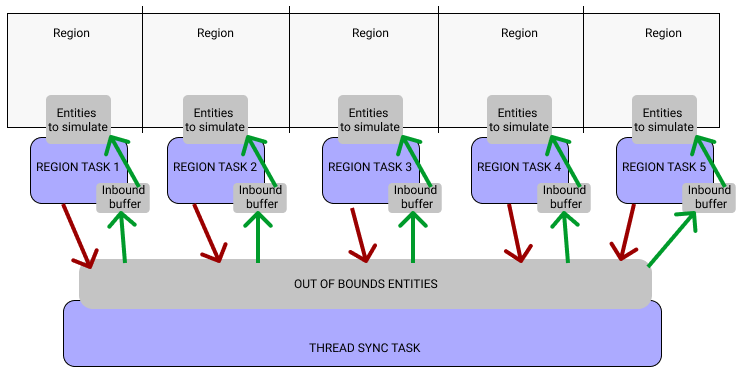
\includegraphics[scale=0.5]{images/multithreaded-layout.png}
	\caption{Reģionu sadalījums plaknei}
	\label{img:multithreaded-layout}
\end{figure}


Izvēle izveidot ,,inbound" buferi Reģioniem radās tādēļ, lai nerastos situācija,
ka entītiju simulācijas brīdī (kur tiek veikta iterēšana pār entītijiem) pēkšņi
rastos kaut kādas modifikācijas un \emph{undefined behaviour}.

Izvēle dalīt visu simulācijas laukumu reģionos pa \(x\) asi (varēja būt arī \(y\)
ass, tikai ne abas asis reizē), bija tāpēc, lai ērti varētu to pielāgot dažādu
kodolu skaitam -  sadalīt plakni \(n\) vienāda platuma un garuma daļās, lai
katram Reģionam būtu vienāds darbības laukums nepāra skaitļiem varētu rast zināmas problēmas.

Darba autors \textbf{neizmanto visus pieejamos procesora kodolus}, jo šādā gadījumā
procesors tiek pārslogots un netiek veikta responsīva UI updeitošanās (par to
vēlāk tiks aprakstīts) -- tāpēc tiek izmantota tiaki \(\frac{2}{3}\) no
pieejamajiem procesora kodoliem (vai sliktākajā gadījuma 1 kodols). Šī iemesla dēļ
\ref{img:multithreaded-layout} attēlā ir parādīti 5 reģioni/5 taski/ \(\frac{2}{3}\) no 8 kodolu sistēmas.

Lai gan, ņemot vērā, ka \(1 Task\neq 1 Thread\), jo Taski izpildās uz .NET Runtime
pieejama threadpoola\cite{csharp:tasks-not-threads}, tad reāli definēt vairāk
Tasksus arī ir iespējams -- runtime definētie threadi (mēdz saukt arī par
\emph{green threads}\cite{progr:green-threads}) izpildās
userspace\cite{sys:userspace}, nevis sistēmas kerneļa līmenī, kas .NET Runtime
atļauj pašam izlemt, kad darīt \emph{concurrent vai paralēlas}\cite{csharp:concurrent-parallel} darbības.
Tasku menedžošana
\emph{userspacā} ir daudz ātrāka nekā zemā līmeņa kerneļa threadu veidošana un izsaukšāna, atļaujot OS to menedžot.
Visi \emph{tasku} dalītie resursi tiek ,,aizsargāti" ar \emph{Mutex}\cite{csharp:mutex}
instancēm, kas garantē to, ka informācija (aizsargātais mainīgias) netiks vienlaicīgi lasīta/rakstīta no
vairākiem threadiem vienlaicīgi, datu integritāte tiek saglabāta. Izstrādes procesā
pareiza Mutex implementācija radīja daudzas kļūdas -- data races un deadlocks.

% CHAPTER LINQ un Pipeline
\subsubsection*{Pipeline}

Lai sistēmā varētu nodrošināt funkciju modularitāti -- karantīna slimajiem,
definēti kopīgie saskarsmes punkti, zombie mode, utt. -- bija nepieciešams
izplānot kādā veidā šo funkcionalitāti varētu ieslēgt un izslēgt koda izpildes
laikā. Darba autors izvēlējās funkciju kompozīcijas dizaina modeli --
\emph{Pipelines}\cite{progr:pipelines}. Pirms tiek izveidota galvenā simulāciajs
instance \emph{World}(\emph{World.cs}), ir jāinicializē \emph{List} ar
\emph{Pipeline} (\emph{BasePipeline.cs}, skat. \ref{img:pipeline-iface})
interfeisa implementējošām instancēm. Interfeisa definīcija apskatāma sekojošajā kodā:

{
\setstretch{1}
\begin{minted}{CSharp}
    public interface Pipeline
    {
        void updateTimeScale(float timeScale);
        PipelineReturnData pushThrough(
            List<EntityOnMap<SickEntity>> currentSick,
            List<EntityOnMap<HealthyEntity>> currentHealthy,
            ulong timeDeltaMs
        );
    }
\end{minted}
}

Objekts \emph{PipelineReturnData}, kuru atgriež \emph{pushThrough} funckija ir
uzskatāms par \emph{type alias} \emph{Tuple<T, K>} mainīgajam

{
\setstretch{1}
\begin{minted}{CSharp}
(List<EntityOnMap<SickEntity>>, List<EntityOnMap<HealthyEntity>>)
\end{minted}
}

, jo C\# nepiedāvā valodas konstrukcij, kas atļautu definēt
\emph{type alias}. Šajā gadījumā tas tika darīts, lai kods būtu lasāmāks.

Talāk atliek tikai veidot klases, kas implementē šo interfeisu -- katrai sistēmas
nepieciešamajai darbībai jāveido sava klases ar interfeisa implementāciju. Kopā
tika izveidoti 8 dažādi \emph{pipeline} objekti:

\begin{enumerate}
    \item AttractorPipeline -- definē rutīnas entītijiem, vietas uz kuriem visi kopīgi dosies.
    \item DeathPipeline -- izņem entītiju no saraksta, ja tā dzīvības ir sasniegušas 0.
    \item GeoLocationPipeline -- ,,kustina" entītiju kartē, aprēķinot tā jauno
        atrašanās vietu, zinot entītija virzienu, ātrumu, esošo lokāciju un pagājušo
        laiku kopš iepriekšējā pipeline izsaukuma.
    \item InfectionPipeline -- pārbauda kuri veselie entītiji ir blakus slimajam
        entītijam un pārkonvertē tos uz jauniem slimniekiem.
    \item QuarantinePipeline -- visus slimos entītijus novieto noteikta plaknes
        stūrī, lai izslimotu savu slimību.
    \item RecoveryPipeline -- ja slimais entītijs ir atveseļojies, tad pārkonvertē to uz veselo entītiju.
    \item TickingPipeline -- ,,padzen" entītija iekšejo pulksteni uz priekšu (pārrēķina jaunu kustības virzienu, veselības stāvokli).
    \item ZombieModePipeline -- liek visiem slimajiem entītijiem dzīties pakaļ vistuvākajam veselajam entītijam.
    \item AssertionPipeline -- \emph{runtime} pārbaude vai visi entīija tipi ir
        pareizi sadalīti (iepriekš komanda izmantoju bet gan dinamisku datu tipu
        kāstošanu \emph{runtime} laikā ar tipu kāstošanu, tāpēc šis pipeline bija
        noderīgs priekš kļūdu izķeršanas).
\end{enumerate}

Sistēmas izstrādes laikā ir jāpievērš arī pipeline secībai, jo katrs pipeline
operē ar iepriekšējā pipeline modificētajiem datiem -- izmainot secību
(vai arī izslēdzot/ieslēdzot kādu) var raasties dažādi iznākumi.

Katrai sistēmas \emph{Region} instancei ir pieejams inicializētais \emph{List<Pipeline>}
objekts, tad ar \emph{LINQ} palīdzību \emph{Region} izpildes ciklā tā iekšējos entītijus
,,izpūš" cauri (\emph{Region.cs} failā):

{
\setstretch{1}
\begin{minted}{CSharp}
    var current = sw.ElapsedMilliseconds;
    var timeDeltaMS = (ulong)(current - previous);
    /* Iterē cauri visiem pipeliniem */
    var pipelineResult = pipelines.Aggregate(new PipelineReturnData
    {
        // Inicializē ar sākotnējām Region vērtībām
        newHealthy = populationHealthy,
        newSick = populationSick
    },
    (aggregate, pipeline) => pipeline.pushThrough(
        aggregate.newSick, aggregate.newHealthy, timeDeltaMS
        )
    );

    // Saglabā izmainītās vērtības
    populationSick = pipelineResult.newSick;
    populationHealthy = pipelineResult.newHealthy;
\end{minted}
}

Papildus uzsvars uz \emph{LINQ} izmantošanu šajā darba aprakstā netiks uzsvērts,
jo tas tika izmantots pilnībā visās \emph{Pipeline} implementācijās, gandrīz vai
visās simulāciajs funkcijas un pat UI saskarnē. Tika izmantotas dažādas šis
funkcionālas paradigmas metodes -- \emph{Aggregate, Where, Select, ForEach, Concat, Min, Max, u.c.}.


\subsubsection{,,frontendserver" pakotne}

% Blazor UI kontrolē pipelines un instanciēšanu

Lietotaju saskarne ir programmēta ar \emph{Blazor} ietvaru. Sākotnēji darba
autors vēlējas izmantot \emph{Blazor WebAssembly} \emph{dotnet template} versiju,
lai varētu visu projektu kā SPA\cite{progr:SPA} uz statiskā faila servera. Tomēr
pašreizējā Blazor versija nepiedāvā vairāku procesu paralelizācijas iespējas
(tikai \emph{concurrent} iespējamību, izmantojot vienu threadu, kas arī ir
izmantots priekš pārlūkprogrammas UI zīmēšanas)\cite{csharp:blazor-no-multithreaded-support}. Lai gan
visi WEB brosweri kopš 2020 gada vasaras atbalsta \emph{WebAssembly Threads}
priekšlikumu \cite{wasm:threads-proposal}, tomēr to ir nepieciešams atsevišķi
,,ieslēgt" caur pārlukprogrammas iestatījumiem. Kā arī \emph{Blazor WebAssembly} neatbalsta vairāku
sistēmas \emph{threadu} izveidi. Šī iemesla dēļ tika izmantots \emph{Blazor Server}
versija, kur visa UI apstrāde (arī simulācijas palaišana) notiek \textbf{uz servera}. Šāda
pieeja gan nozīmē, to, ka reāli uz serveriem šo sistēmu likt nav laba doma -- jo
vairāk cilvēkie pieslēgsies un veiks simulācijas, jo lielāka slodze. Tomēr tā ir
problēma ārpus šī kursadarba ietvariem.

% Canvas pakotne
Pati attēla zīmēšana tiek veikta ar uz \emph{HTML5 Canvas} elementa\cite{html5:canvas}.
Šis elements piedāvā JavaScript API, lai zīmētu rēala laika grafikas, attēlus, animācijas.
Tiek piedāvāti dažādi veidi kādu API izmantot -- ,,2d", ,,webgl", ,,webgl2",
,,bitmaprenderer" \cite{html5:canvas-contexts}. Tomēr šie ir JavaScript API, lai
no C\# tos izsauktu, ir nepieciešams izveidot ,,wrapper" funkcijas šim JS API,
nodrošinot starp-valodu komunikāciju. Tomēr ir jau izveidots Blazor extensions,
kas nodrošina šo JavaScript API wrapper funckijas -- \emph{BlazorExtensions.Canvas}
(\url{https://github.com/BlazorExtensions/Canvas}).
Darba autors jau iepriekš bija darbojies ar WebGL, kas nodrošinātu ātru un efektīvu
zīmējuma veidošanu un atjaunināšanu, tomēr šī \emph{BlazorExtensions.Canvas} bibliotēkas
dokumentācijā aprakstītais WebGL piemērs nestrādāja -- tāpēc darba izstrādē tika
izmantots ,,2d" context API.

% Data polling
Ņemot vērā, inicializējot un uzstartējot simulāciju, tā faktiski iet atsevišķā
sistēmas threadā, tad no lietotāju saskarnes puses nav viens konkrēts moments, kad
varētu iegūt visas nepieciešamās vērtības par esošajiem entītijiem sistēmā. Risinājums
ir izmantot tādu kā \emph{data polling}\cite{progr:data-polling}. Koda sekvences
diagrammu ir iespējams aplūkot \ref{img:squance-diagram-get-status} attēlā. Katrā
datu pieprasījuma reizē ir nepieciešams nopauzēt (iekšējais mainīgais, kas raksturo esošo stāvokli) visas \emph{Region} instances,
lai nenotiktu \emph{data races}, nepieciešams nopauzēt pašu \emph{World} instanci (lai
,,OutOfBounds" sinhronizācija nenotiktos datu nolases brīdī), tad nepieciešams apkopot
datus no visām datu krātuvēm, atpauzēt visas instances, atgriezt datus lietotāju saskarnei.

\begin{figure}[H]
	\centering
	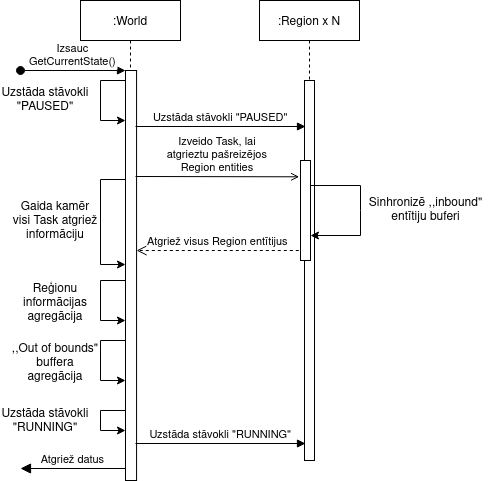
\includegraphics[scale=0.7]{images/DiseaseCore-GetData.png}
	\caption{Simulācijas datu stāvokļa vaicājuma izpilde}
	\label{img:squance-diagram-get-status}
\end{figure}

Tālāk šie iegūtie dati Blazor pusē tiek papildus sadalīti: metadati tiek nodoti
\emph{Statistics} komponentei, kas aprēķina katra \emph{Region} ātrdarbību, bet
reāli dati par entītiju stāvokļiem tiek nodota \emph{Canvas} komponentei, kur
entītiji tiek sašķiroti un katrs uzzīmēts uz \emph{HTML canvas}.
